\chapter{Applications}

\section{Graph Laplacian Matrix}
For a directed graph, we can use incidence matrix to represent it.
The row of the matrix represents an edge, the column of it represents a vertex.

\begin{example}
    Suppose we have a graph which can be represented in this diagram:

    \begin{center}
        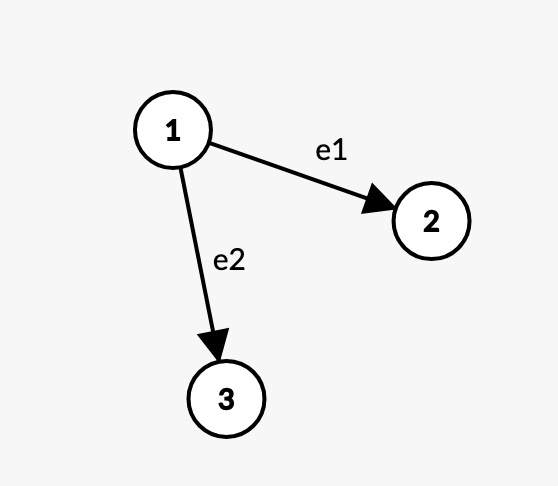
\includegraphics[width=0.4\textwidth]{DAG}
        \captionof{figure}{A simple directed acyclic graph}
        \label{fig:simpel-dag}
    \end{center}

    The incidence matrix will be:
   \[
        C = \begin{bmatrix}
            1& -1 & 0 \\
            1 & 0 & -1 \\
        \end{bmatrix}
   \] 

   The 1st row of the matrix represents edge \(e_1\), where arrow from vertex 1 to vertex 2; the 2nd row of the matrix represents edge \(e_2\), where arrow from vertex 1 to vertex 3. 

   The Laplacian matrix can be represented as:
    \[
        L(G) = C^T C
    \]

    Do the math:
    \[
        C^T C = 
        \begin{bmatrix}
            1 &  1 \\
            -1 &  0 \\
            0 &  -1 \\
        \end{bmatrix}
        \begin{bmatrix}
            1 & -1 &  0 \\
            1 & 0 &  -1 \\
        \end{bmatrix}
        =
        \begin{bmatrix}
            2 & -1 &  -1 \\
            -1 & 1 &  0 \\
            -1 & 0 &  1 \\
        \end{bmatrix}
    \] 

    Here are some observations:
    \begin{itemize}
        \item The diagonal numbers show the degree of each vertex: for example, vertex 0 has 2 edges.
        \item The non-diagonal numbers show the edge between different vertices. For example, row1-column2/ row2-column1 both show that vertex 1 and vertex 2 have one edge.
        \item Notice that the direction disappears in the Laplacian matrix.
    \end{itemize}

    \textbf{For Diagonal Values: }

    For vertex 1, \(\begin{bmatrix}
        1 &  1 \\
    \end{bmatrix}\) represents vertex 1's position in each of the arrows, because it is the starter of both \(e_1\) and \(e_2\), so both elements are \(1\).  

    The result of \(\begin{bmatrix}
        1 &  1 \\
    \end{bmatrix} 
    \begin{bmatrix}
         1 \\
         1 \\
    \end{bmatrix}
    = 2\) 
    is a sum of squares, thus will always be greater or equal to 0. 

    The sum represents the degree of the vertex.

    \textbf{For Non-diagonal Values: }

    For vertex 2 (\(v_2\) ), \(\begin{bmatrix}
        -1 &  0 \\
    \end{bmatrix}\) represents that it is the receiver in \(e_1\)(thus -1), and it does not involve in \(e_2\)(thus -1).  

    For the same reason, vertex 3 (\(v_3\) ) can be represented by \(\begin{bmatrix}
        0 &  -1 \\
    \end{bmatrix}\).

    We have \(v_2 v_3^T = 0\) meaning those 2 vertices have no common edge.  
\end{example}

To generalize the idea, a Laplacian Matrix can be viewed as the remainder of a diagonal matrix representing degree of each vertex and a matrix representing the presence of each edge:
\[
    L(G) = C^TC = D - W
\]

For example, the Laplacian Matrix of the above example can be written as:
\[
    \begin{bmatrix}
        2 & -1 &  -1 \\
        -1 & 1 &  0 \\
        -1 & 0 &  1 \\
    \end{bmatrix}
    =
    \begin{bmatrix}
        2 & 0 &  0 \\
        0 & 1 &  0 \\
        0 & 0 &  1 \\
    \end{bmatrix} 
    -
    \begin{bmatrix}
        0 & 1 &  1 \\
        1 & 0 &  0 \\
        1 & 0 &  0 \\
    \end{bmatrix}
\]



